
\pdfoutput=1
\documentclass[11pt]{article}

% Final version generation
% \usepackage[review]{acl}
\usepackage[]{acl}
\usepackage{graphicx}
\usepackage[caption=false]{subfig}


% Standard package includes
\usepackage{times}
\usepackage{latexsym}

% Latin characters
\usepackage[T1]{fontenc}

% UTF8 Encoding 
\usepackage[utf8]{inputenc}

% Space saver
\usepackage{microtype}

\title{
Vardial 2022 shared task: Italian dialect Identification (Project proposal)\\
\vspace{0.2cm}
\small Computational Semantics for NLP, Spring 2022
}

\author{
Quynh Anh Nguyen,
Giacomo Camposampiero 
\and Francesco Di Stefano \\         
ETH Zurich - Swiss Federal Institute of Technology \\ \texttt{\{quynguyen, gcamposampie, fdistefano\}@ethz.ch}
}

\begin{document}
\maketitle

\section{Introduction}\label{sec:intro}
Dialect classification represents a key task in the improvement of many other downstream tasks such as opinion mining and machine translation, where the enrichment of text with geographical information can potentially result in improved performances for real-world applications \cite{zampieri_nakov_scherrer_2020}.

As a result, the interest in the study of language variation has been steadily growing in the last few years, as highlighted by the increasing number of publications and events related to the topic.
However, little has been done so far by researchers in the context of automatic dialect recognition for the Italian language.

In this context, the \textit{Languages and Dialects of Italy} (ITDI) task of VarDial Evaluation Campaign 2022\footnote{The website will be publicly available from end of April.} aims to bridge this gap, facilitating the development of models capable of properly classifying 11 regional languages and dialects from both Italy's mainland and islands (Piedmontese, Venetian, Sicilian, Neapolitan, Emilian-Romagnol, Tarantino, Sardinian, Ligurian, Friulian, Ladin, Lombard).

The shared task organizers provide a dataset consisting of a large pool of Wikipedia articles written in one of these dialects, in the form of Wikipedia dump.
The task is closed and, therefore, participants are not allowed to use external data to train their models (exception done for off-the-shelf pre-trained language models from the HuggingFace model hub or similar, the use of which however has to be clearly stated). 

The predictions are evaluated at sentence level using $F_1$ score. %the shared task  

\section{Related works}
In this section, we will briefly introduce several methods \cite{zampieri_nakov_scherrer_2020} which used to be applied on classification problems on similar languages or different dialects of a language.
        \paragraph{Italian dialect identification SoTa}
        For what concerns Italian dialect identification, there are several researches working on analysing Italian dialects features \cite{DBLP:journals/corr/abs-2010-05993} but no previous experiments deal with language identification task is found. Thus, our scope is to find a way to tackle this problem drawing inspiration from related works in dialect identification in different languages rather than overcome a particular state of the art model. In particular, we aim to obtain good results with the use of deep neural networks, more specifically adopting CNN and transformer architectures.
        \paragraph{Machine learning models vs CNN}
        Although deep learning models yield state of the art performances in many NLP tasks, an ensemble of SVM and Naive Bayes models was the best performing model in the Uralic Language Identification task in the VarDial Evaluation Campaign 2021 \cite{ceolin-2021-comparing}. \emph{Linear SVM} classifier, \emph{Naive Bayes} model, the combination of the two methods \emph{Linear SVM + Naives Bayes} as well as \emph{CNN} were implemented to  classify target languages. Three machine learning approaches were all trained on TF-IDF character n-grams. The experiment shows that CNN did not always outperform the other machine learning approaches.
        %Moreover, the experiment also reveals that shuffling improved the performance of the CNN on the language identification task of Romanian and Moldavian which are quite closed to Italian dialects.

        \paragraph{CNN}
        Even if the state of the art in many dialect identification tasks has been reached through the application of transformer-based models, the use of CNNs is still high in this type of task. In particular, taking as an example the Romanian vs Moldavian dialect, CNN-based approaches achieved competitive results in both VarDial 2019 Evaluation Campaign \cite{tudoreanu-2019-dteam} and VarDial 2020 Evaluation Campaign \cite{Rebeja2020ADS}.%.we have excellent results with CNNs in the VarDial 2019 Evaluation Campaign \cite{tudoreanu-2019-dteam} and the VarDial 2020 Evaluation Campaign \cite{Rebeja2020ADS}
        
        \paragraph{Transformer}
        The introduction of transformers \cite{NIPS2017_3f5ee243} has revolutionized many tasks in NLP and the identification of dialects isn't an exception. Models based on this architecture achieved state-of-the-art results in many application. A recent example is again VarDial 2020 Evaluation Campaign, where the use of a fine-tuned version of BERT previously trained on three publicly available Romanian corpora \cite{zaharia-etal-2020-exploring} reached a weighted $F_1$ score of $96.25 \%$ on the MOROCO dataset \cite{moroco} in the Romanian vs Moldavian identification task. 
        
\section{Dataset}% Giacomo
As already mentioned in the section \ref{sec:intro}, the training dataset is provided by the organizers and consists of $265 \, 016$ selected Wikipedia articles from 1st March 2022 dumps. 
As the training data is provided in the form of raw Wikipedia dumps, careful pre-processing of the data is part of the task.
The development and test sets have not been disclosed yet, and will be made available to the participants according to the task milestones reported in Section \ref{sec:milestones}.

Since the data doesn't come from a well-know documented dataset, a preliminary exploration has been initially conducted to gain useful insight about it. This investigation highlighted a huge imbalance between classes as shown in Figure \ref{fig:dist}, since the 3 most represented dialect (Venetian, Piedmontese and Lombard) account for almost three quarters of the entire articles in the training data.
However, as shown in Figure \ref{fig:len}, the number of articles per dialect might not be fully representative on itself, since the size of each articles has also to be taken in account. This is the case of Lombard dialect, for example, which accounts for a large portion of training articles ($19\%$), but more than a quarter of them are not longer than 2 sentences.

Nonetheless, imbalanced data seems to represent the main challenge posed by this dataset and should be addressed during the evaluation of the model.
%Nonetheless, since the evaluation metric is F1 score which takes in account the class imbalance, \emph{imbalanced data} 
%Through the above analysis, we figure out that \emph{imbalanced data} could be the main challenge to achieve the great performance since the evaluation metric is F1 score. 
Possible solutions to the problem are data augmentation, weighted modelling and data sub-sampling.


\begin{figure}[h]
\centering
\subfloat[Distribution of Wikipedia articles across dialects.]{%
    \centering
    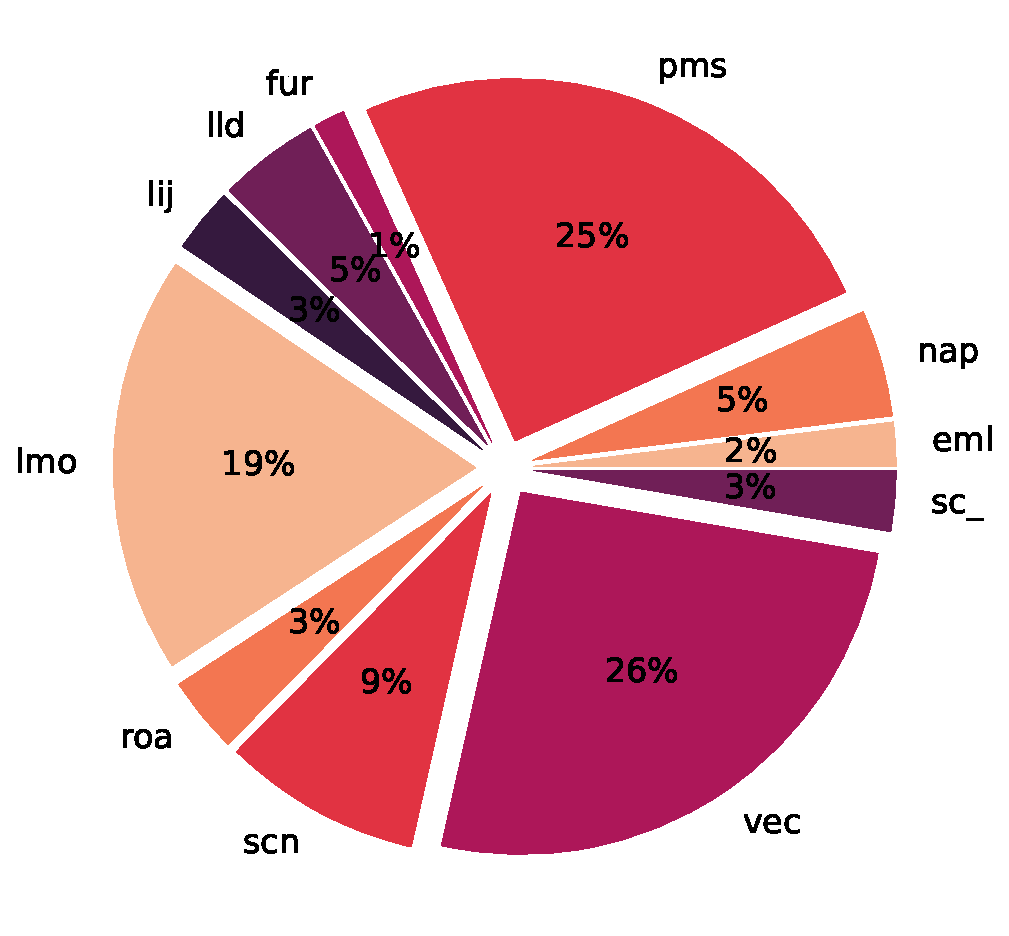
\includegraphics[clip, width=0.9\columnwidth]{figures/figure1.pdf}
    \label{fig:dist}
}
\hfill
\subfloat[Number of sentences of articles in the training set, grouped by dialect.]{%
    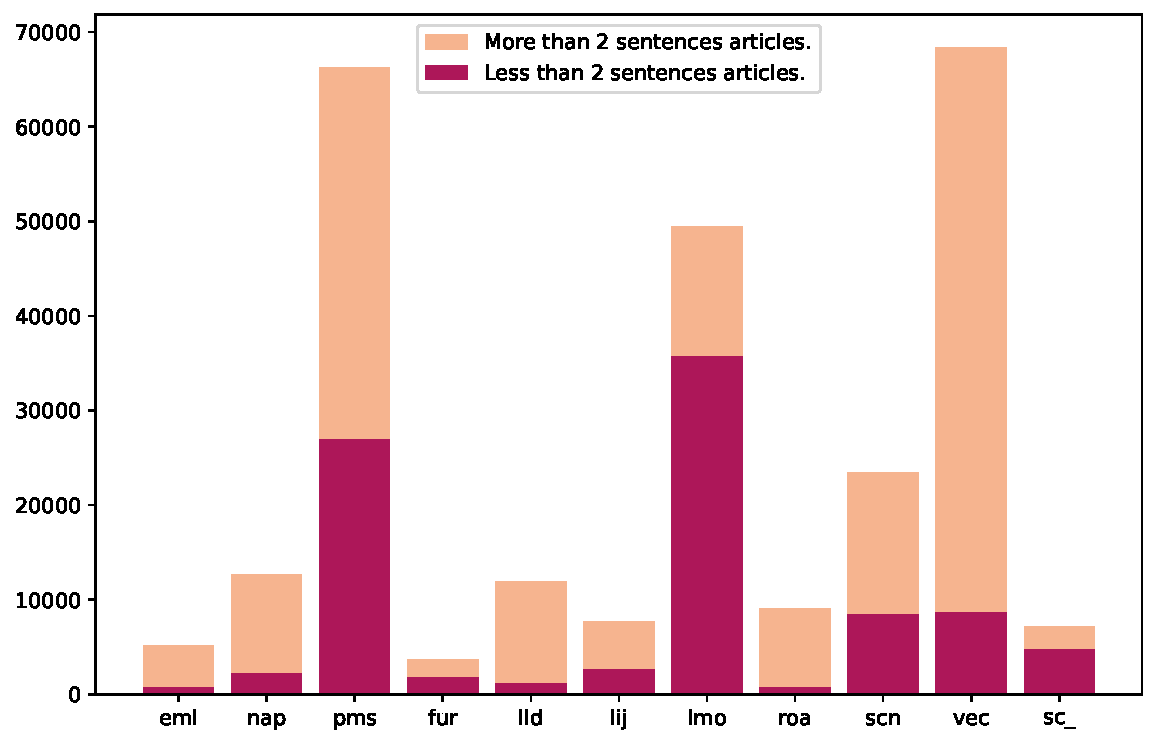
\includegraphics[clip, width=.9\columnwidth]{figures/figure2.pdf}
    \label{fig:len}
}
\caption{Preliminary data exploration on training set.}
        \label{fig:dataexpl}
\end{figure}
    \section{Approaches} \label{sec:appr}
        In order to tackle the Italian dialect identification tasks, we plan to investigate different approaches, including Machine Learning methods and Deep learning methods.
        \paragraph{ML approaches} Linear SVM and Naive Bayes are the two methods which are still popularly used to handle this specific task. Thus, we would like to implement them with tf$-$idf character n-grams varying from 3 to 5 grams as in the experiment of \cite{ceolin-2021-comparing}. These approaches could be also used as baseline models to compare to deep neural network approaches such as CNN or Transformers.
        \paragraph{CNN} %Which approach with CNN?
        Convolutional Neural Networks were employed with success by many teams in the previous editions of the dialect identification task. Therefore, we plan to experiment with a classifier that uses a CNN for feature extraction on top of an embedding layer - that could be a skip-gram model \cite{10.5555/2999792.2999959} as in the case of \cite{tudoreanu-2019-dteam}.  
        
        \paragraph{Transformer} As said above, the use of transformer-based models yield state of the art results even in the task of dialect identification. In particular, the fine-tuning of pre-trained versions of BERT obtained good results in this field. Following this line, our approach with this type of model would be to adopt a version of BERT pre-trained with the Italian language \cite{PolignanoEtAlCLIC2019} and to fine-tune this latter on our task.


\section{Expected Result} % anh
The main objective of this project is twofold.
\begin{itemize}
    \item To develop a model based on the approaches described in Section \ref{sec:appr}; the resulting model should output sufficiently correct and consistent predictions to eventually allow our group to make a submission to the shared task.
    \item To gain useful insights about the resulting model, through ablation studies and error analysis. 
\end{itemize}
Besides, since we participate to a shared task, we hope to achieve a good rank in the task leader board.

\section{Milestones}
\label{sec:milestones}
The timeline outlined by the organizers is defined as follows.
\begin{enumerate}
    \item \textit{Now}: Training set and task description are already provided.
    \item \textit{End of April}: The shared task will be published in the Vardial 2022 website and will officially start. The development set will be disclosed.
    \item \textit{End of June}: The system should be finished.
    \item \textit{End of July}: deadline to submit the system description paper.
\end{enumerate}

% Entries custom bib
\bibliography{custom}
\bibliographystyle{acl_natbib}

% \appendix
% \section{Example Appendix}
% \label{sec:appendix}
% In case we need an appendix.

\end{document}